
%%%%%%%%%%%%%%%%%%%%%%%%%%%%%%%%%%%%%%%%%%%%%%%%%%%%%%%%%%%%%%%%%%%%%%%%%%%%%%%%
%   Document
%
\begin{document}

% Title page
\maketitle

\frontmatter
\section*{Acknowledgements}
The author thanks Professor Christopher Nielsen for his guidance in developing the required intuition and mathematical tools for path following control design. Plots and simulations were partly written in Mathworks MATLAB under a student licence. Other simulations were written using C++ linked with the Boost library~\cite{boost} and Catch test framework~\cite{catch}.

\begin{flushright}
Rollen S. D'Souza\\
Software Engineering\\
University of Waterloo\\
\texttt{rs2dsouz@edu.uwaterloo.ca}
\end{flushright}

\tableofcontents

\printnomenclature[3cm]
\listoffigures
\listoftables

%\cleardoublepage
%\phantomsection
%\addcontentsline{toc}{chapter}{Acronyms and Initialisms}
%\printglossary[title=Acronyms and Initialisms]

%%%%%%%%%%%%      MAIN MATTER      %%%%%%%%%%%%
\mainmatter
\pagestyle{fancy}
\renewcommand{\sectionmark}[1]{\markright{\thesection.\ #1}}

\chapter{Introduction}

\section{Background}
A common control objective for mobile robots involves tracking a trajectory in the space the robot operates in. This space is known as the task space of the robot, denoted as $\mathcal{T}$. Often the structure of this space is unknown --- along with the goal --- and the robot must first explore the world using an exploration and mapping algorithm before deciding on a goal and path.  This paper is concerned with a restricted subset of this problem. Consider a differential drive robot starting at location $(0,0)\in\mathcal{T}$, placed in a world with an unknown number of obstacles, that is given the objective to reach position $(x,y)$ in task space without colliding with obstacles. A two-pronged approach can be taken to safe-guard from collisions:
\begin{enumerate}
    \item Plan a path that can be followed successfully by the robot and does not intersect with any obstacles for all future time.
    \item Design a controller that ensures sufficiently fast convergence to the path and provides a guarantee, under reasonable assumptions, that the robot will not leave the path.
\end{enumerate}
Planning a path is a field in its own right. The most practical, and dominant, philosophy to path planning involves sampling $\mathcal{T}$ and incrementally building a path to the goal region. The sampling algorithm used is critical to performance and effective coverage of $\mathcal{T}$. If the sampling technique does not adequately sample the space in question the algorithm may take considerably longer to generate a path that reaches $\mathcal{G}$. Incorporated in these algorithms is the ability to test the feasibility of a path. For example, whether any collisions would occur with the known environment and whether any differential constraints of the robot are broken. For example, the robot cannot turn instantaneously. This addition ensures that unfeasible paths are rejected early instead of wasting time developing a path that is known to be unfeasible. Of course, the astute reader notes that this type of path generation often creates discrete segments that lead to the goal. There are techniques in literature to develop smooth paths incrementally in coordination with a sampling algorithm but these are considered outside the scope of this work \cite{Yang14}. Other advanced approaches to generate smooth paths rely on the construction of a vector field over $\mathcal{T}$ \cite{LaValle06} but these are also relatively complicated algorithms.

Instead this report takes a simpler approach that generates a smooth function out of the discrete waypoints produced by the relatively simple Rapidly exploring Randomized Tree (RRT) algorithm. The smooth function generated is a polynomial spline, a stitched sequence of possibly distinct polynomials that preserves a set of continuity conditions at the stitch-points. After generation, the spline is tested again for feasibility before being propagated to the controller. There are apparent performance issues in this approach addressed in Section \ref{sec:planning}.

Independently the field of non-linear control theory developed techniques to follow arbitrary paths. Standard control techniques tend to yield poor results in tracking a path. A number of techniques in literature exist to drive a robot towards a path and converge upon it. However, most of these techniques do not provide invariance once on the path~\cite{Gill15}. This lack of invariance reduces the robustness of the technique as the controller may not stay on the path even under perfect environmental conditions! This motivated the development of a new family of path following controllers that treat the path as an invariant set that is then stabilized through linear control, described in Section \ref{sec:control}. This family of controllers use transverse feedback linearization to reformulate the problem and assist in constructing a linear controller that compensates for the non-linearities imposed by the path. This report discusses a few methods to planning and control for the purpose of driving a differential drive robot towards a goal.

\section{Notation and Report Organization}
\nomenclature{$\mathcal{T}$}{Mobile robot task space.}
\nomenclature{$\mathcal{T}_{(w,h)}$}{Rectangular mobile robot task space with width $w$ and height $h$.}
\nomenclature{$\vec{x}$}{A vector in $\R^n$.}
\nomenclature{$\vec{x}_i$}{The $i$-th component of vector $\vec{x}$}
\nomenclature{$\mat{M}$}{A matrix. Can be assumed real unless stated otherwise.}
\nomenclature{$\mat{M}_{(i,j)}$}{The value at the $i$-th row and $j$-th column of matrix $\mat{M}$. The variables may have a $:$ substituted to indicate selection of all values in that dimension, similar to that found in the Matlab grammar.}
This report assumes proficiency in multi-variable calculus and basic control theory. Any results taken from theory of dynamical systems and other advanced undergraduate mathematical courses are stated and cited from a source used by the author. Scalars are denoted as $x$, vectors as $\vec{x}$ and matrices as $\mat{X}$. Time derivatives are denoted using Newton's dot notation and any other derivatives are denoted using primes if the independent variable is clear and Leibniz notation otherwise. In practice, planning algorithms generally precede control. However this report instead defers discussion of planning until after describing control methodologies in Section \ref{sec:control}. This content placement is intended to give the reader a better intuition for the decisions made at planning stage.

\section{Problem Statement}
Let the task space, without loss of generality, be the rectangular space  $\mathcal{T}_{(\bar{x},\bar{y})} = \{(x,y)\in\mathbb{R}^2 : 0 \leq x \leq \bar{x} \wedge 0 \leq y \leq \bar{y}\}$. For simplicity, consider the kinematic model of a differential drive robot with the combined position and orientation state vector $\vec{x}=\trans{(x,y,\theta)}\in\R^3$. The robot has a controllable forward velocity $v\in\R$ and a controllable turning rate $u\in\R$. $v$ is assumed to be positive.
\begin{figure}[!htbp]
    \centering
    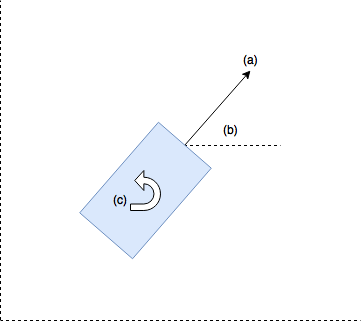
\includegraphics[width=3in]{images/diffdrive_kin_model.png}
    \caption{Kinematic model of differential drive robot. (a) is the direction vector along which the robot is currently facing, denoted by $\vec{g}_v$. That is a function of $x_3$, the angle of the vector with respect to $x$-axis which is shown at (b). (c) is the rate at which the robot turns and is controlled by $u$.}
    \label{fig:basic_kinematic_model}
\end{figure}
The kinematic system dynamics are
\begin{align}
    \mat{G}(\vec{x}) &=
        \begin{bmatrix}
            0 & \cos(\vec{x}_3)\\
            0 & \sin(\vec{x}_3)\\
            1 & 0
        \end{bmatrix}
        =
        \begin{bmatrix}
            \vec{g}_u & \vec{g}_v
        \end{bmatrix} \nonumber \\
    \dot{\vec{x}} &=
        \mat{G}(\vec{x})
        \begin{bmatrix} u \\ v \end{bmatrix}.
    \label{eqn:basic_kinematic_model}
\end{align}
The robot must at some unspecified finite time arrive at a given goal region $\mathcal{G}\subset\mathcal{T}$. Note there is no restriction in how it arrives in this region other than it does so safely. Starting at time $t=0$ and then at a regular time interval $\Delta$, the robot observes the world and decides, based on the observation, whether a new plan is required to approach the goal region. This may occur when the robot observes a new obstacle that the robot's currently planned path intersects. The simplest and most widely used planning algorithms involve the generation of a tree that explores the current model of the world. This family of algorithms generate a sequence of waypoints. From planning stage a path $\vec{\sigma}: [0,1]\subset\R\to\mathcal{T}$ with $\vec{\sigma}(1)\in\mathcal{G}$ is generated.

The path $\vec{\sigma}_a$ is fed into the path following control which guides the robot over time towards, and along, the path in order to arrive in $\mathcal{G}$. Further, the control algorithm must converge towards the path in a manner that is both guaranteed and as fast as possible. It must also faithfully follow the path in order to reduce the chances of re-planning. Given that the robot may not have a perfect model of the world, i.e, is not aware of all obstacles, a re-plan may still occur. The planning algorithm is required to design a new $\vec{\sigma}_b$ so as to preserve any properties the control algorithm requires to stay on the trajectory continuously.

\chapter{Control}\label{sec:control}
Three control strategies are considered for path following. The simplest controller, in terms of design and implementation, is the point-chasing controller. The other two techniques rely on the approach of transverse feedback linearization which decomposes the path following problem into transverse and tangential dynamical systems. This section assumes the path is of the form in \eqref{eqn:quintic}. The matrix representation of a quintic polynomial is chosen for succinct representation.
\begin{align}
    &\mat{P}\in\R^{2\times6} \nonumber \\
    &\vec{\sigma}(\lambda) =    \mat{P}
                                \begin{bmatrix}
                                    1 \\
                                    \lambda^1 \\
                                    \lambda^2 \\
                                    \lambda^3 \\
                                    \lambda^4 \\
                                    \lambda^5
                                \end{bmatrix}.
    \label{eqn:quintic}
\end{align}

\section{Trajectory Controller}\label{sec:trajectory}
\begin{figure}[!htbp]
    \centering
    \includegraphics[width=4in]{images/trajectory_model.png}
    \caption{Visual description for trajectory controller. (a) is the scaled direction vector $l\vec{\tau}$ that is then added to the current position and compared to the point (b) tracing the curve.}
    \label{fig:basic_traj_vis}
\end{figure}
A trajectory controller involves treating the parameter $\lambda$ of the path $\vec{\sigma}$ as a function of time, $t$, and designing a controller that converges to this moving point. In order to apply this strategy, the control is designed around a point that leads the robot's current position. Let the observation be defined as,
\begin{align*}
    \mat{H} &= \begin{bmatrix} 1 & 0 & 0 \\ 0 & 1 & 0 \end{bmatrix}\\
    \vec{\tau} &= \begin{bmatrix} \cos(\vec{x}_3) \\ \sin(\vec{x}_3) \end{bmatrix} \\
    \vec{y}_l &= \mat{H}\vec{x} + l\vec{\tau}(\vec{x}_3)
\end{align*}
for some positive $l\in\R$. We let $\vec{y}_{ref}(t) = \vec{\sigma}\left(\lambda(t)\right)$. This is visually shown in Figure \ref{fig:basic_traj_vis}. The introduction and restriction of the parameter $l$ is made clear in the controller derivation. Define the position error $\vec{e} \defineas \vec{y}_l - \vec{y}_{ref}$ and take the time derivative to form a new dynamical system in terms of the path error,
\begin{align*}
    \dot{\vec{e}}   &= \dot{\vec{y}}_l - \dot{\vec{y}}_{ref}\\
                    &= \mat{H}\left(\vec{G}(\vec{x})\begin{bmatrix} u \\ v \end{bmatrix}\right) + l\dot{\vec{\tau}} - \vec{\sigma}'(\lambda(t))\dot{\lambda}(t)\\
                    &= \begin{bmatrix} v~cos~\vec{x}_3 \\ v~sin~\vec{x}_3 \end{bmatrix}
                        +
                        \begin{bmatrix} -l~sin\vec{x}_3 \\ l~cos~\vec{x}_3 \end{bmatrix} u
                        -
                        \vec{\sigma}'(\lambda(t))\dot{\lambda}(t)\\
                    &=  \begin{bmatrix}
                            -l~\sin\vec{x}_3 & \cos~\vec{x}_3 \\
                            l~\cos~\vec{x}_3 & \sin~\vec{x}_3 \\
                        \end{bmatrix}
                        \begin{bmatrix}
                            u \\ v
                        \end{bmatrix}
                        -
                        \vec{\sigma}'(\lambda(t))\dot{\lambda}(t). \numberthis \label{eqn:traj_error_dynamics}
\end{align*}
At this point the reader may observe that the matrix multiplying the control signals is invertible if and only if $l$ is non-zero. We now construct a controller of the form
\begin{align*}
    \begin{bmatrix}
        u \\ v
    \end{bmatrix}   &=  \begin{bmatrix}
                            -l~\sin\vec{x}_3 & \cos~\vec{x}_3 \\
                            l~\cos~\vec{x}_3 & \sin~\vec{x}_3 \\
                        \end{bmatrix}^{-1}
                        \left[
                            \mat{K}\vec{e} + \vec{\sigma}'(\lambda(t))\dot{\lambda}(t)
                        \right].
\end{align*}
Notice that this choice of controller yields $\dot{\vec{e}}=\mat{K}\vec{e}$ when substituting into \eqref{eqn:traj_error_dynamics}, forming a closed loop linear system. As long as $\mat{K}\in\R^{2\times 2}$ is Hurwitz, the closed loop system is stable. As a simplification, this paper assumes $\lambda(t)=\frac{t}{T_f}$ where $T_f > 0$ is some constant scaling factor.

\section{Transverse Feedback Linearization}
A variety of techniques were designed to address the issues observed in the point chasing controller. One of these techniques is transverse feedback linearization. Transverse feedback linearization is the mathematical reformulation of system dynamics into transverse and tangential components with respect to the closest point to the path. This restatement of the problem allows for the capturing of the path dynamics --- combining that with the original system dynamics --- and permits cancellation of non-linearities introduced by the path as it affects the system.

The technique was generalized in \cite{Nielsen06} for aperiodic paths and then further expanded in \cite{Hladio13}. The approaches defined in those works restricted their design to following simple curves, such as circles. Gill et al., in \cite{Gill15}, applied the technique to a larger class of paths, specifically splines in $C^p$ with $p>=2$. Note that their work is not restricted to polynomial splines and in fact applies to any functions that are stitched at waypoints preserving $C^p$ continuity on the whole parameterized domain as well as requiring derivatives up to order $p$ be linearly independent. As stated previously, it is assumed in this work that these splines are quintic polynomials in order to provide a relevant benchmark comparison.

\subsection{General Form}\label{sec:general_tfl}
Recall the kinematic model for a differential drive robot, from \eqref{eqn:basic_kinematic_model}. Unlike the trajectory controller, this controller will assume that $v$ is a fixed quantity. Therefore, the system dynamics may be rearranged into
\begin{align*}
    \dot{\vec{x}} &=
        \vec{g_v}(\vec{x})
        v
        +
        \vec{g_u}
        u \\
    &\defineas \vec{f}(\vec{x}) + \vec{b} u. \numberthis \label{eqn:tfl_kinematic_system}
\end{align*}
The output of the system is defined as
\begin{align*}
    \mat{H} &= \begin{bmatrix} 1 & 0 & 0 \\ 0 & 1 & 0 \end{bmatrix}\\
    \vec{y}(\vec{x}) &= \mat{H}\vec{x}.
\end{align*}
As before, let the path be $\vec{\sigma}:[0,1]\to\mathcal{T}\subset\R^2$ and $C^2$ everywhere. A few regularity condition are required.
\begin{assumption}[Path is self-intersection free]
    \begin{equation*}
        \forall \lambda_1, \lambda_2 \in\R : \vec{\sigma}(\lambda_1) = \vec{\sigma}(\lambda_2) \Leftrightarrow \lambda_1 = \lambda_2
    \end{equation*}
    \label{ass:self_intersect}
\end{assumption}
\begin{assumption}[Path is a regular curve.]
    \begin{equation*}
        \forall \lambda\in\R : \vec{\sigma}'(\lambda) \neq 0
    \end{equation*}
    \label{ass:regular}
\end{assumption}
Take note that there is no restriction on the domain of $\vec{\sigma}$ in the assumptions although work in this report does restrict the domain. We define a new state vector $\vec{\xi} \defineas \trans{(\vec{\xi}_1, \vec{\xi}_2)}$ where $\vec{\xi}_1$ is left undefined for now. One may view $\vec{\xi}_1$ as the signed tracking error of the robot with respect to the path. The variation of this state is what differentiates the variety of techniques used. When the path is well known and simple --- such as a circular arc --- this state may be expressed in closed form. This is not always the case. Let us then define $\vec{\xi}_2 \defineas \dot{\vec{\xi}}_1$. Chain rule gives,
\begin{align*}
    \vec{\xi}_2     &=  \dot{\vec{\xi}}_1\\
                    &=  \der{\vec{x}}\vec{\xi}_1 \dot{\vec{x}}\\
                    &=  \der{\vec{x}}\vec{\xi}_1
                        \begin{bmatrix}
                            v~cos(\vec{x}_3)\\
                            v~sin(\vec{x}_3)\\
                            u
                        \end{bmatrix}.
\end{align*}
Under the assumption that this error is independent of robot heading we can further simplify the expression such that $\vec{\xi}_2=\der{\vec{x}}\vec{\xi}_1 \vec{f}(\vec{x}) \rdefineas \lie{\vec{f}}\vec{\xi}_1(\vec{x})$. The function $\lie{\vec{f}}\vec{\xi}_1 : \R^3\to\R$ is known as the Lie derivative of $\vec{\xi}_1$ along the vector field $\vec{f}(\vec{x})$. Notice the control signal has no impact on our state. The lack of a control signal in the dynamical system motivates finding the time derivative of $\vec{\xi}_2$. Using properties of Lie derivatives, it is not difficult to show that $\vec{\xi}_2=\lie{\vec{b}}\lie{\vec{f}}\vec{\xi}_1(\vec{x}) u + \lie{\vec{f}}^2 \vec{\xi}_1(\vec{x})$. This yields the system dynamics,
\begin{equation}
    \vec{\dot{\xi}}
    =
    \begin{bmatrix}
        \xi_2 \\
        \lie{\vec{b}}\lie{\vec{f}}\vec{\xi}_1(\vec{x}) u + \lie{\vec{f}}^2 \vec{\xi}_1(\vec{x})
    \end{bmatrix}.
    \label{eqn:tfl_dynamics}
\end{equation}
\eqref{eqn:tfl_dynamics} can be solved for the control signal. Motivated by the structure of \eqref{eqn:tfl_dynamics}, we take our control law to be
\begin{equation}
    u = \frac{ u_{aux} - \lie{\vec{f}}^2 \vec{\xi}_1(\vec{x}) }{ \lie{\vec{b}}\lie{\vec{f}}\vec{\xi}_1(\vec{x}) },
    \label{eqn:tfl_general_control}
\end{equation}
where $u_{aux}$ is an outer loop control signal that is yet to be defined. The reader may wonder under what conditions $\lie{\vec{b}}\lie{\vec{f}}\vec{\xi}_1(\vec{x})$ is non-zero. This is not apparent, although intuition may guide us. Since $\lie{\vec{b}}\lie{\vec{f}}\vec{\xi}_1(\vec{x})$ scales the control signal we expect it to vanish whenever the control signal has no instantaneous impact on the change in the orthogonal error. This may occur, for example, when the differential robot is facing towards the nearest point. Leaving the discussion of singularities aside, we set $u_{aux} \defineas \trans{\vec{k}}\vec{\xi}$ with $\vec{k}\in\R^2$. Substituting $u_{aux}$ into \eqref{eqn:tfl_general_control} and \eqref{eqn:tfl_dynamics}, the partial dynamical system becomes
\begin{equation}
    \dot{\vec{\xi}}
    =
    \begin{bmatrix}
        0 & 1\\
        \vec{k}_1 & \vec{k}_2 \\
    \end{bmatrix}
    \vec{\xi}.
    \label{eqn:tfl_control_dynamics}
\end{equation}
This system only describes dynamics transversally as we have no control over $v$ in the original system. \eqref{eqn:tfl_control_dynamics} is a linear system that is stable as long as the gains $\vec{k}_1$ and $\vec{k}_2$ are negative, as per the Routh-Hurwitz criterion.

\subsection{Sylvester Approach}
The Sylvester methodology relies on the theoretical developments of elimination theory. Elimination theory investigates the theoretical methods that discover common roots of polynomials. The essential idea is to reformulate \eqref{eqn:quintic} into a system of homogeneous linear equations that has a non-trivial kernel \cite{Sederberg84}. This non-trivial kernel allows for the derivation of an implicit representation of the path, otherwise known as a level set, that can then be stabilized by the transverse feedback linearization. First, we state a necessary result from linear algebra.
\begin{theorem}
    Let $\mat{A}\in\R{n\times n}$ and $\vec{x}\in\R^n$. Then the solution to $\mat{A}\vec{x}=\vec{0}$ is non-unique if and only if $\det\mat{A}=0$. \label{thm:kernel}
\end{theorem}
Notice that if we formulate a new system from \eqref{eqn:quintic} that is square and homogeneous, we will be able to eliminate $\vec{\lambda}$ by instead considering when $\det\mat{A}=0$ for some constructed $\mat{A}$. This is otherwise known as finding the resultant~\cite{Sederberg84}. Homogenizing the path requires treating $\vec{\sigma}_1$ and $\vec{\sigma}_2$ as constants $\vec{y}_1$ and $\vec{y}_2$, moving them into the polynomial matrix $\mat{P}$. We call this modified matrix $\mat{Q}$. With this modification, we need only construct a square system out of $\mat{Q}$. In order to construct a square linear system, we consider multiplying both polynomials in the first and second component of $\vec{\sigma}$ by increasing powers of $\lambda$ until we have generated a sufficient number of equations. For two quintics, we must multiply the polynomials by powers of $\lambda$ up til $\lambda^5$, arriving at \eqref{eqn:inhomog_poly}. The matrix $S$ and its determinant are known as the Sylvester matrix and the Sylvester resultant respectively.
\begin{equation}
    \begin{bmatrix}
        & \mat{Q}_{1:} & \vec{0}_{1\times 6} \\
        0 & \mat{Q}_{1:} & \vec{0}_{1\times 5} \\
        \vec{0}_{1\times 2} & \mat{Q}_{1:} & \vec{0}_{1\times 4} \\
        \vec{0}_{1\times 3} & \mat{Q}_{1:} & \vec{0}_{1\times 3} \\
        \vec{0}_{1\times 4} & \mat{Q}_{1:} & \vec{0}_{1\times 2} \\
        \vec{0}_{1\times 5} & \mat{Q}_{1:} & \vec{0}_{1\times 1} \\
        \vec{0}_{1\times 6} & \mat{Q}_{1:} & \\
        & \mat{Q}_{2:} & \vec{0}_{1\times 6} \\
        0 & \mat{Q}_{2:} & \vec{0}_{1\times 5} \\
        \vec{0}_{1\times 2} & \mat{Q}_{2:} & \vec{0}_{1\times 4} \\
        \vec{0}_{1\times 3} & \mat{Q}_{2:} & \vec{0}_{1\times 3} \\
        \vec{0}_{1\times 4} & \mat{Q}_{2:} & \vec{0}_{1\times 2} \\
        \vec{0}_{1\times 5} & \mat{Q}_{2:} & \vec{0}_{1\times 1} \\
        \vec{0}_{1\times 6} & \mat{Q}_{2:} & \\
    \end{bmatrix}
    \begin{bmatrix}
        1 \\
        \lambda^1 \\
        \lambda^2 \\
        \lambda^3 \\
        \lambda^4 \\
        \lambda^5 \\
        \lambda^6 \\
        \lambda^7 \\
        \lambda^8 \\
        \lambda^9 \\
        \lambda^{10} \\
        \lambda^{11}
    \end{bmatrix}
    =
    \mat{S}(\vec{y})\vec{\lambda}.
    \label{eqn:inhomog_poly}
\end{equation}
Carefully note that the tail of $\mat{Q}_{1:}$ and $\mat{Q}_{2:}$ contain a linear term in $\vec{y}_1$ and $\vec{y}_2$ respectively. Therefore if the matrix has a non-trivial kernel, i.e. its determinant vanishes as per \eqref{thm:kernel}, both $\vec{y}_1$ and $\vec{y}_2$ satisfy the polynomial equations. This motivates the definition of the zero level set, $s(\vec{y}) = \det\mat{S}(\vec{y})$. This can be expressed as a function of $\vec{x}$ as,
$$
    (s\circ \vec{y})(\vec{x}) = \det\mat{S}(\mat{H}\vec{x}).
$$
The method assumes the matrix $\mat{S}$ does not have a trivially vanishing determinant such as if the leading coefficients of both polynomials $\vec{\sigma}_1$ and $\vec{\sigma}_2$ are equal. In that case, extensions to the method exist that allow for the factoring of these terms~\cite{Sederberg84}. Now we can define $\vec{\xi}_1$, the distance from the robot to the path, as the level set function $\vec{\xi}_1 \defineas (s\circ \vec{y})(\vec{x})$. Observe that $\vec{\xi}_1$ is only dependent on $\vec{x}_1$ and $\vec{x}_2$. Define $\vec{\xi}_2 \defineas \dot{\vec{\xi}}_1 = \der{\vec{y}}s~\mat{H}\vec{f}(\vec{x})$. To complete the control system, we must differentiate $\vec{\xi}_2$ in time. We expect \eqref{eqn:tfl_dynamics} to emerge.
\begin{align*}
    \dot{\vec{\xi}}_2   &=  \frac{d}{dt}\left[\der{\vec{y}}s\right]\mat{H}\vec{f}(\vec{x})
                            +
                            \der{\vec{y}}s\frac{d}{dt}\left[\mat{H}\vec{f}(\vec{x})\right]\\
                        &=  \trans{\left(\mat{H}\vec{f}(\vec{x})\right)}\frac{d}{dt}\trans{\left[\der{\vec{y}}s\right]}
                            +
                            \der{\vec{y}}s\frac{d}{dt}\left[\mat{H}\vec{f}(\vec{x})\right]\\
                        &=  \trans{\left(\mat{H}\vec{f}(\vec{x})\right)}\left[\der{\vec{y}}^2 s\right]\mat{H}\vec{f}(\vec{x})
                            +
                            \left(\der{\vec{y}} s\right)\mat{H}\frac{\partial\vec{f}}{\partial\vec{x}}\vec{b}u\\
                        &= \lie{\vec{f}}^2 \xi_1(\vec{x}) + \lie{\vec{b}}\lie{\vec{f}}\xi_1(\vec{x})~u
\end{align*}
The controller implementation follows from Section \ref{sec:general_tfl}.

\subsection{Serret-Frenet Frame Approach}
\nomenclature{$\Rot{\theta}$}{Counter-clockwise rotation matrix in $\R^2$ of angle $\theta$.}
\nomenclature{$B_\epsilon(\vec{x})$}{Open ball of radius $\epsilon$ centred about $\vec{x}$ in the appropriate vector space.}
First we must impose an extra regularity condition, in addition to \eqref{ass:self_intersect}, in order for this controller to work.
\begin{assumption}[Existence and Uniqueness of Nearest Point]
    Let $C\defineas\vec{\sigma}([0,1])$. There exists an open, connected set $\mathcal{U}\subset\mathcal{T}$ such that,
    \begin{equation*}
        (\forall y\in\mathcal{U}) : (\exists \lambda_* \in [0,1]) : \forall \lambda\in[0,1], \lambda\neq\lambda_* : \enorm{y - \sigma(\lambda_*)} < \enorm{y - \sigma(\lambda)}.
    \end{equation*}
    \label{ass:unique_operating}
\end{assumption}
The path parameter $\lambda_*$ is the nearest point on the curve to the robot. It is not difficult to see that this point also has the property that $\vec{\sigma}'(\lambda_*)$ is orthogonal to the error. A linear basis that spans $\R^2$ is built from $\lambda_*$. Let the first basis vector $\vec{e}_1 \defineas \vec{\sigma}'(\lambda_*)/(\enorm{\vec{\sigma}'(\lambda_*)})$. The second basis vector can be formed through a 90 degree rotation, such that $\vec{e}_2 \defineas \Rot{\frac{\pi}{2}}\vec{e}_1$. These basis vectors form the Serret-Frenet basis that spans $\R^2$. Relying on the intuition of previous derivations, we let $\vec{\xi}_1 \defineas \trans{\vec{e}_2}\left(\vec{h}(\vec{x}) - \vec{\sigma}(\lambda_*)\right)$. In words $\vec{\xi}_1$ is the orthogonal tracking error with respect to the closest point on the curve. We complete the (partial) dynamical system state by differentiating $\vec{\xi}_1$ to find $\vec{\xi}_2$,
\begin{align*}
    \vec{\xi}_2     &=  \dot{\vec{\xi}}_1\\
                    &=  \trans{\dot{\vec{e}}_2}\left(\vec{h}(\vec{x}) - \vec{\sigma}(\lambda_*)\right)
                        +
                        \trans{\vec{e}_2}\left(\mat{H}(\vec{f}(\vec{x}) + \vec{g}u) - \vec{\sigma}'(\lambda_*)\dot{\lambda} \right)\\
                    &=  \trans{\dot{\vec{e}}_2}\left(\vec{h}(\vec{x}) - \vec{\sigma}(\lambda_*)\right)
                        +
                        \trans{\vec{e}_2}\left(\mat{H}(\vec{f}(\vec{x}) + \vec{g}u) - \vec{\sigma}'(\lambda_*)\dot{\lambda} \right).
\end{align*}
We require a result from differential geometry in order to continue.
\begin{definition}[Curvature]
    The curvature of a regular, $C^2$ curve $\sigma:\R\to\R^2$ is
    \begin{equation}
        \kappa(\lambda) = \frac{\enorm{\vec{\sigma}''(\lambda) \times \vec{\sigma}'(\lambda)}}{\enorm{\vec{\sigma}'(\lambda)}^3}
    \end{equation}.
\end{definition}
Our definition of the basis vectors as well as the restriction to planar curves (curves in $\R^2$) allows for a simplified definition of the curvature,
\begin{lemma}[Signed Curvature of Planar Curve with Serret-Frenet Basis]
    The signed curvature is
    $$\kappa(\lambda) = \frac{\trans{\vec{\sigma}''(\lambda)}\vec{e}_2}{\enorm{\vec{\sigma}'(\lambda)}^2}.$$
    \label{lem:signed_curvature}
\end{lemma}
\begin{proof}
    Let $\theta$ be the angle between $\vec{\sigma}$ and $\vec{e}_1$.
    \begin{align*}
        \kappa(\lambda) &= \frac{\enorm{\vec{\sigma}''(\lambda) \times \vec{\sigma}'(\lambda)}}{\enorm{\vec{\sigma}'(\lambda)}^3}\\
                        &= \frac{\enorm{\vec{\sigma}''(\lambda) \times \vec{e}_1}}{\enorm{\vec{\sigma}'(\lambda)}^2}\\
                        &= \frac{\left|\enorm{\vec{\sigma}''(\lambda)}\sin \theta \right|}{\enorm{\vec{\sigma}'(\lambda)}^2}\\
                        &= \frac{\left|\trans{\vec{\sigma}''(\lambda)}\vec{e}_2\right|}{\enorm{\vec{\sigma}'(\lambda)}^2}.\\
    \end{align*}
\end{proof}
The curvature describes how much the curve's tangent changes. This is necessary to describe succinctly the derivative of the basis vectors. One more result will allow us to derive the derivatives of the basis vectors.
\begin{lemma}
    Let $\vec{v}_1, \vec{v}_2:\R\to S^1$ such that both are $C^2$. Additionally, let $\vec{v}_2(\lambda)=\Rot{\frac{\pi}{2}}\vec{v}_1(\lambda)$. Then, the derivatives of the vectors are related by a (parameter-varying) scalar multiple of the opposing vector such that
    \begin{align*}
        \vec{v}'_1(\lambda) &= \gamma(\lambda)\vec{v}_2 \\
        \vec{v}'_2(\lambda) &= -\gamma(\lambda)\vec{v}_1.
    \end{align*}
    \label{lem:sf_frame}
\end{lemma}
\begin{proof}
    Observe that $\forall \lambda\in\R : \trans{\vec{v}_1(\lambda)}\vec{v}_1(\lambda)\equiv 1$. Differentiating gives $\trans{\vec{v}'_1}\vec{v}_1=0$. Since $\{\vec{v}_1,\vec{v}_2\}$ spans $\R^2$, $\trans{\vec{v}'_1}=\gamma(\lambda)\vec{v}_2$. It is worth mentioning that $\gamma\in C^1$. The derivative $\vec{v}'_2$ follows similarly with the substitution $\vec{v}_2(\lambda)=\Rot{\frac{\pi}{2}}\vec{v}_1(\lambda)$.
\end{proof}
\begin{corollary}[Derivative of Serret-Frenet Frame]
    For $\vec{e}_1$ and $\vec{e}_2$ as defined for the Serret-Frenet Controller,
    \begin{align*}
        \vec{e}'_1(\lambda) &= \kappa(\lambda)\enorm{\vec{\sigma}'(\lambda)}\vec{e}_2 \\
        \vec{e}'_2(\lambda) &= -\kappa(\lambda)\enorm{\vec{\sigma}'(\lambda)}\vec{e}_1
    \end{align*}.
    \label{cor:der_frame}
\end{corollary}
\begin{proof}
    Differentiate $\vec{e}_1$ with respect to $\lambda$ explicitly,
    \begin{align*}
        \frac{d\vec{e}_1}{d\lambda} &=  \frac{d}{d\lambda}\left[ \frac{\vec{\sigma}'(\lambda)}{\enorm{\vec{\sigma}'(\lambda)}}\right]\\
                                    &=  \frac{1}{\enorm{\vec{\sigma}'(\lambda)}^2}\left[\vec{\sigma}''(\lambda)\enorm{\vec{\sigma}'(\lambda)}-\vec{\sigma}'(\lambda)(\enorm{\vec{\sigma}'(\lambda)})^{-1}\trans{\vec{\sigma}''(\lambda)}\vec{\sigma}'(\lambda)\right]\\
                                    &=  \frac{1}{\enorm{\vec{\sigma}'(\lambda)}}\left[\vec{\sigma}''(\lambda)-(\trans{\vec{\sigma}''(\lambda)}\vec{e}_1)\vec{e}_1 \right]\\
                                    &=  \frac{1}{\enorm{\vec{\sigma}'(\lambda)}}\left[\trans{\vec{\sigma}''(\lambda)}\vec{e}_2\right]\vec{e}_2
    \end{align*}
    Likening the result with \eqref{lem:sf_frame} and \eqref{lem:signed_curvature}, we see the statement is proven.
\end{proof}
A generalization of \eqref{lem:sf_frame} exists in higher dimensions and can be found in any modern differential geometry text~\cite{Kuhnel06}. \eqref{cor:der_frame} permits the elimination of the first and last terms in $\vec{\xi}_2$. In practice, it may not always be possible to use --- or even find --- the closest point $\lambda_*$ and therefore there may be some error introduced in the system dynamics. An analysis of this effect is performed later. For now, we discard this term and observe that the vector $\vec{b}$ is in the kernel of $\vec{H}$ yielding a simple expression for $\vec{\xi}_2$,
$$\vec{\xi}_2 = \trans{\vec{e}_2}\mat{H}\vec{f}(\vec{x})$$
This definition may be intuitively described as the projection of the output on the orthogonal vector. Define a new state vector $\vec{\xi}$ as before. Once again we would like to take the time derivative of $\vec{\xi}_2$ to complete the dynamical system. However two more Lemmas are required to help us take the time derivative of the basis vectors.
\begin{lemma}
    There exists a function $\varpi:\mathcal{U}\to[0,1]$ that generates the operating point $\lambda_*$ from the position of the robot (the observation). The derivative of $\varpi$ along the solutions of the system,
    $$\der{\vec{y}}\varpi(\vec{y}) = \frac{\trans{\vec{e}_1}}{\enorm{\vec{\sigma}'(\lambda_*)}}.$$
\end{lemma}
\begin{proof}
    Refer to Gill~\cite{Gill15}.
\end{proof}
Computing the derivative of $\vec{\xi}_2$ we find,
\begin{align*}
    \dot{\vec{\xi}}_2
                &=  \trans{\dot{\vec{e}}_2}\mat{H}\vec{f}(\vec{x})
                    +
                    \trans{\vec{e}_2}\mat{H}\frac{\partial\vec{f}}{\partial\vec{x}}\left[\vec{f}(\vec{x}) + \vec{b}u\right]\\
                &=  \trans{(\mat{H}\vec{f}(\vec{x}))}\dot{\vec{e}}_2
                    +
                    \trans{\vec{e}_2}\mat{H}\frac{\partial\vec{f}}{\partial\vec{x}} \vec{b} u \\
                &=  \trans{(\mat{H}\vec{f}(\vec{x}))}\vec{e}'_2\left[(\der{\vec{y}}\varpi)\mat{H}\vec{f}(\vec{x}) \right]
                    +
                    \trans{\vec{e}_2}\mat{H}\frac{\partial\vec{f}}{\partial\vec{x}} \vec{b} u \\
                &=  \trans{(\mat{H}\vec{f}(\vec{x}))}\left[-\kappa(\lambda_*)\left(\enorm{\vec{\sigma}'(\lambda_*)} \right)\right]\vec{e}_1\left[(\der{\vec{y}}\varpi)\mat{H}\vec{f}(\vec{x})\right]
                    +
                    \trans{\vec{e}_2}\mat{H}\frac{\partial\vec{f}}{\partial\vec{x}}\vec{b} u\\
                &=  -\trans{(\mat{H}\vec{f}(\vec{x}))}\vec{e}_1 \frac{\trans{\vec{\sigma}''(\lambda)}\vec{e}_2}{\enorm{\vec{\sigma}'(\lambda)}}\frac{\trans{\vec{e}_1}\mat{H}\vec{f}(\vec{x})}{\enorm{\vec{\sigma}'(\lambda_*)}}
                    +
                    \trans{\vec{e}_2}\mat{H}\frac{\partial\vec{f}}{\partial\vec{x}}\vec{b} u\\
                &=  -\left[\trans{\vec{e}_1}\mat{H}\vec{f}(\vec{x})\right]^2 \frac{\trans{\vec{e}_2}\vec{\sigma}''(\lambda)}{\trans{\vec{\sigma}'(\lambda)}\vec{\sigma}'(\lambda_*)}
                    +
                    \trans{\vec{e}_2}\mat{H}\frac{\partial\vec{f}}{\partial\vec{x}}\vec{b} u\\
                &=  \lie{\vec{f}}^2\vec{\xi}_1(\vec{x}) + \lie{\vec{b}}\lie{\vec{f}}\vec{\xi}_1(\vec{x}) u.
\end{align*}
This result completes the partial dynamical system and allows for the construction of the linear controller. However, we would like to simplify the above system to be in terms of only $\vec{\xi}$, if possible. A useful result that combines the knowledge of our model and formulation of the basis vectors is required.
\begin{lemma}
    The translational velocity of the robot may be decomposed through projections on the basis vectors,
    $$
        v = \sqrt{ \left(\trans{\vec{e}_2}\mat{H}\vec{f}(\vec{x})\right)^2 + \left(\trans{\vec{e}_1}\mat{H}\vec{f}(\vec{x})\right)^2 }
    $$
    which implies that,
    $$
        \left(\trans{\vec{e}_1}\mat{H}\vec{f}(\vec{x})\right) = \sqrt{v^2 - \vec{\xi}_2^2}.
    $$
\end{lemma}
\begin{proof}
    The result follows from the fact that $\{ \vec{e}_1, \vec{e}_2 \}$ form an orthonormal basis and that $v = \enorm{\mat{H}\vec{f}(\vec{x})}$.
\end{proof}
\begin{align*}
    \dot{\vec{\xi}}_2 &=
                    -\left[\trans{\vec{e}_1}\mat{H}\vec{f}(\vec{x})\right]^2  \frac{\trans{\vec{e}_2}\vec{\sigma}''(\lambda)}{\trans{\vec{\sigma}'(\lambda)}\vec{\sigma}'(\lambda_*)}
                    +
                    \trans{\vec{e}_2}\mat{H}\frac{\partial\vec{f}}{\partial\vec{x}}\vec{g} u\\
                &=
                    -\left(v^2 - \vec{\xi}_2^2\right) \frac{\trans{\vec{e}_2}\vec{\sigma}''(\lambda)}{\trans{\vec{\sigma}'(\lambda)}\vec{\sigma}'(\lambda_*)}
                    +
                    \trans{\vec{e}_2}\mat{H}\frac{\partial\vec{f}}{\partial\vec{x}}\vec{g} u\\
                &=
                    -\left(v^2 - \vec{\xi}_2^2\right) \frac{\trans{\vec{e}_2}\vec{\sigma}''(\lambda)}{\trans{\vec{\sigma}'(\lambda)}\vec{\sigma}'(\lambda_*)}
                    +
                    \trans{\vec{e}_2}
                        \begin{bmatrix}
                            -v~\sin x_3 \\
                            v~\cos x_3
                        \end{bmatrix}
                    u\\
                &=
                    -\left(v^2 - \vec{\xi}_2^2\right) \frac{\trans{\vec{e}_2}\vec{\sigma}''(\lambda)}{\trans{\vec{\sigma}'(\lambda)}\vec{\sigma}'(\lambda_*)}
                    +
                    \trans{\vec{e}_2}\Rot{\frac{\pi}{2}}
                        \begin{bmatrix}
                            v~\cos x_3 \\
                            v~\sin x_3
                        \end{bmatrix}
                    u\\
                &=
                    -\left(v^2 - \vec{\xi}_2^2\right) \frac{\trans{\vec{e}_2}\vec{\sigma}''(\lambda)}{\trans{\vec{\sigma}'(\lambda)}\vec{\sigma}'(\lambda_*)}
                    +
                    \trans{\vec{e}_2}\Rot{\frac{\pi}{2}}\vec{H}\vec{f}(\vec{x}) u\\
                &=
                    -\left(v^2 - \vec{\xi}_2^2\right) \frac{\trans{\vec{e}_2}\vec{\sigma}''(\lambda)}{\trans{\vec{\sigma}'(\lambda)}\vec{\sigma}'(\lambda_*)}
                    +
                    \trans{\left(\Rot{-\frac{\pi}{2}}\vec{e}_2\right)}\vec{H}\vec{f}(\vec{x}) u\\
                &=
                    -\left(v^2 - \vec{\xi}_2^2\right) \frac{\trans{\vec{e}_2}\vec{\sigma}''(\lambda)}{\trans{\vec{\sigma}'(\lambda)}\vec{\sigma}'(\lambda_*)}
                    +
                    \trans{\vec{e}_1}\mat{H}\vec{f}(\vec{x}) u\\
                &=
                    -\left(v^2 - \vec{\xi}_2^2\right) \frac{\trans{\vec{e}_2}\vec{\sigma}''(\lambda)}{\trans{\vec{\sigma}'(\lambda)}\vec{\sigma}'(\lambda_*)}
                    +
                    u \sqrt{v^2 - \vec{\xi}_2^2}.\\
\end{align*}
We now construct a general control signal of the form
\begin{equation*}
    u = \frac{u_{aux} + \left(v^2 - \vec{\xi}_2^2\right) \frac{\trans{\vec{e}_2}\vec{\sigma}''(\lambda)}{\trans{\vec{\sigma}'(\lambda)}\vec{\sigma}'(\lambda_*)}}{\sqrt{v^2 - \vec{\xi}_2^2}}
\end{equation*}
Notice that $\left|\vec{\xi}_2\right|$ must never equal $v$. Intuitively this means that the robot's speed must not be completely represented in the orthogonal direction --- towards the path. This concern motivates an analysis on whether stability may be guaranteed while avoiding singularities in the control law at $\left|\vec{\xi}_2\right|=v$. Like in previous sections, we once again choose $u_{aux} = \trans{\vec{k}}\vec{\xi}$ and observe that this forms a closed loop linear system of the exact same form as \eqref{eqn:tfl_control_dynamics}. Again, the gains $\vec{k}_1$ and $\vec{k}_2$ need to be negative to ensure stability of the closed loop dynamics. However, this result doesn't guarantee the system will not encounter the singularity described above. In summary, the robot's partial dynamics for the Serret-Frenet controller is,
\begin{equation*}
    \dot{\vec{\xi}} =
        \begin{bmatrix}
            \vec{\xi}_2 \\
            -\left(v^2 - \vec{\xi}_2^2\right) \frac{\trans{\vec{e}_2}\vec{\sigma}''(\lambda)}{\trans{\vec{\sigma}'(\lambda)}\vec{\sigma}'(\lambda_*)}
        \end{bmatrix}
        +
        \begin{bmatrix}
            0 \\
            \sqrt{v^2 - \vec{\xi}_2^2}
        \end{bmatrix}
        u
\end{equation*}

\subsubsection{Stability Analysis and Control Design}\label{sec:sf_stability_analysis}
The final control system, with proportional linear feedback, is
\begin{equation}
    \vec{\dot{\xi}} =   \begin{bmatrix}
                            0 & 1 \\
                            \vec{k}_1 & \vec{k}_2
                        \end{bmatrix}
                        \vec{\xi}.
    \label{eqn:tfl_linear}
\end{equation}
We begin with a necessary result from Dynamical System Theory.
\begin{theorem}[Positive Invariance]
    Let $\Omega\subset\R^2$ be an open, connected set and $V:\Omega\to\R$ be continuously differentiable such that $$ \dot{V}(\vec{\xi})\leq 0, \vec{\xi}\in\Omega.$$ Then $\Omega$ is made positively invariant by $V(\vec{\xi})$. That is all orbits that begin in $\Omega$ stay in $\Omega$.
    \label{thm:lasalle}
\end{theorem}
Now we prove the main result,
\begin{theorem}[Singularity-Free Orbits for Serret Frenet Control]
    For any $M>0$, there exists a choice of gains --- $\vec{k}_1$, $\vec{k}_2$ --- such that an open, connected set $\Omega$ is made positively invariant by some Lyapunov function $V(\vec{\xi})$ under the closed loop dynamics of \eqref{eqn:tfl_linear}. Furthermore, the set $\Omega$ has the properties
    \begin{enumerate}
        \item $\sup_{\vec{\xi}\in\Omega}{\left|\vec{\xi}_1\right|} = M$
        \item $\sup_{\vec{\xi}\in\Omega}{\left|\vec{\xi}_2\right|} = v$.
    \end{enumerate}
    \label{thm:sf_stability}
\end{theorem}
\begin{proof}
    We use the method of undetermined coefficients over a quartic positive definite form. Let $V(\vec{\xi}) = \vec{\xi}_1^4 + a\vec{\xi}_1^2\vec{\xi}_2^2 + b\vec{\xi}_2^4$ where $a, b\in\R$ and are positive. We construct $\Omega$ as the open, connected, sub-level set of $V$ so that $\Omega=\left\{\vec{\xi} : V(\vec{\xi}) < D\right\}.$ We would like to impose restrictions on $a$, $b$, $c$, and $D$ so that $\Omega$ is made positively invariant by $V$ and so that $\Omega$ has the desired properties. Impose $b = Dv^{-4}$ to ensure that $\left|\vec{\xi}_2\right| < v$. We attempt to find further conditions so that $\dot{V}<0$,
    \begin{align*}
        \dot{V} &=  4\vec{\xi}_1^3\dot{\vec{\xi}}_1 + 2a\left[\vec{\xi}_1\dot{\vec{\xi}}_1\vec{\xi}_2^2 + \vec{\xi}_1^2\vec{\xi}_2\dot{\vec{\xi}}_2\right] + 4b\vec{\xi}_2^3\dot{\vec{\xi}}_2\\
                    &=  4\vec{\xi}_1^3\vec{\xi}_2 + 2a\left[\vec{\xi}_1\vec{\xi}_2^3 + \vec{k}_1\vec{\xi}_1^3\vec{\xi}_2 + \vec{k}_2\vec{\xi}_1^2\vec{\xi}_2^2\right] + 4b\vec{k}_1\vec{\xi}_1\vec{\xi}_2^3 + 4b\vec{k}_2\vec{\xi}_2^4\\
                    &=  \left(4+2a\vec{k}_1\right)\vec{\xi}_1^3\vec{\xi}_2 + 2\left(a + 2b\vec{k}_1\right)\vec{\xi}_1\vec{\xi}_2^3 + \left(2a\vec{\xi}_1^2\vec{\xi}_2^2 + 4b\vec{\xi}_2^4\right)\vec{k}_2\\
                    &=  \left(4+2a\vec{k}_1\right)\vec{\xi}_1^3\vec{\xi}_2 + 2\left(a + 2Dv^{-4}\vec{k}_1\right)\vec{\xi}_1\vec{\xi}_2^3 + \left(2a\vec{\xi}_1^2\vec{\xi}_2^2 + 4Dv^{-4}\vec{\xi}_2^4\right)\vec{k}_2.\\
    \end{align*}
    Impose the requirement that cross-terms vanish identically. This gives the restrictions on $a$ and $\vec{k}_1$,
    \begin{align*}
        \vec{k}_1 &= -\frac{v^2}{\sqrt{D}}\\
        a &= 2\frac{\sqrt{D}}{v^2}.
    \end{align*}
    Then $V(\vec{\xi}) = \vec{\xi}_1^4 + 2\frac{\sqrt{D}}{v^2}\vec{\xi}_1^2\vec{\xi}_2^2 + \frac{D}{v^4}\vec{\xi}_2^4$. Interestingly, this is the square of a quadratic form. Specifically,
    $$
        V(\vec{\xi}) = \left[\vec{\xi}_1^2 + \left(\frac{\sqrt{D}}{v^2}\right)\vec{\xi}_2^2 \right]^2.
    $$ We now know that $\dot{V} = \left(2a\vec{\xi}_1^2\vec{\xi}_2^2 + 4Dv^{-4}\vec{\xi}_2^4\right)\vec{k}_2$. Now, $\dot{V} < 0$ if $\vec{k}_2 < 0$. We therefore impose $\vec{k}_2 < 0$. $\Omega$ is now made positively invariant as a consequence of \eqref{thm:lasalle}. Specify $D = M^4$ and find
    \begin{align*}
        \sup_{\vec{\xi}\in\Omega}{\left|\vec{\xi}_1\right|} &= M\\
        \sup_{\vec{\xi}\in\Omega}{\left|\vec{\xi}_2\right|} &= v
    \end{align*}
    as required. Substituting the restricted $a$, $b$, $c$, and $D$ back into our equation we find in summary
    \begin{align*}
        \vec{k}_1 &= -\left( \frac{v}{M} \right)^2\\
        \vec{k}_2 &< 0\\
        \Omega &= \left\{ \vec{\xi} : \vec{\xi}_1^2 + \left(\frac{M}{v}\right)^2 \vec{\xi}_2^2 < M^2 \right\}\\
        V(\vec{\xi}) &= \left[\vec{\xi}_1^2 + \left(\frac{M}{v}\right)^2\vec{\xi}_2^2 \right]^2.
    \end{align*}
\end{proof}
\begin{corollary}
    For any $M > 0$, an open, connected set of solutions that have initial conditions that observe
    \begin{equation*}
        \trans{\vec{\xi}(0)}
        \begin{bmatrix}
            1 & 0\\
            0 & \left(\frac{M}{v}\right)^2
        \end{bmatrix}
        \vec{\xi}(0)
        <
        M^2
    \end{equation*}
    will asymptotically converge to $\vec{0}$ without encountering the singularity $\left|\vec{\xi}_2\right|=v$.
    \label{cor:sf_stability}
\end{corollary}
\begin{proof}
    Proof follows from the fact that the closed loop system in \eqref{eqn:tfl_linear} is stable if and only if both gains are negative, which they are in \eqref{thm:sf_stability}.
\end{proof}
Observe that \eqref{cor:sf_stability} \emph{does not} guarantee a singularity-free orbit for all initial conditions using a single choice of gains. It simply states that a certain set, that is chosen a-priori, is made positively invariant by a choice of gain. In fact, if one were to let $M\to\infty$ then the gains will tend to $0$ and the dynamical system degenerates so that closed loop stability is not maintained. Also observe the simplicity of the set $\Omega$ that is constructed. It is easy to test in practice whether or not the system is within the singularity-free region for a particular controller design. This result motivates a control design methodology for the Serret-Frenet controller. By choosing a maximum allowable orthogonal error $M$, the gain $\vec{k}_1 = -(\frac{v}{M})^2$ is determined. Observe that \eqref{eqn:tfl_dynamics} is a second order system with characteristic polynomial $s^2 - \vec{k}_2 s - \vec{k}_1$. Then the harmonic frequency and damping ratio are,
\begin{align*}
    \omega &= \sqrt{-\vec{k}_1}\\
    \zeta &= \frac{-\vec{k}_2}{2 \sqrt{-\vec{k}_1}}.
\end{align*}
\eqref{cor:sf_stability} limits the choice of $\vec{k}_1$ so we can only determine the damping ratio. We would like, for simplicity, to choose to have no overshoot while still optimizing for the fastest convergence. This implies we need $\zeta = \sqrt{2}/2$. This design decision restricts $\vec{k}_2 = -\sqrt{-2\vec{k}_1}$. The implementation used in this paper chooses $M=0.1$ since the controller expects a very little amount of error.

\chapter{Planning}\label{sec:planning}
Path planning involves the generation of waypoints and curves for the purpose of arriving at some goal region, $\mathcal{G}$. This paper only describes the Rapidly exploring Randomized Tree (RRT) algorithm. A majority of the investigation in planning occurred in the polynomial spline generation phase.

\section{RRT}
The Rapidly exploring Randomized Tree (RRT) algorithm is made up of the following steps \cite{Karaman11},
\begin{enumerate}
    \item Initialize tree $R=\{ \vec{x}_0 \}$ with the initial point.
    \item Randomly sample a candidate point $\vec{x} \in \mathcal{T}$.\label{itm:rrt_sample}
    \item Find the nearest point $\vec{x}_n\in \mathcal{T}$ to $x$, based on some metric over $\mathcal{T}$.
    \item Add an edge $(\vec{x}_n, \vec{x})$ if the path between them is collision free.
    \item If $\vec{x}\in\mathcal{G}$ halt, otherwise repeat from (\ref{itm:rrt_sample}).
\end{enumerate}
The tree grows in a random fashion from the initial point, rapidly expanding in $\mathcal{T}$ until the goal can be reached. Once the algorithm completes, the programmer need only back-trace from the goal point towards the initial point; trees have a unique path from any node to the root. There are a few design decisions that can be made here in order to improve performance of the algorithm. One is to store obstacles in what is known as an R-Tree. R-Trees --- a tree whose name stems from rectangle, not rapidly nor randomized --- are a data structure that stores data according to their position in space. R-Tree creates bins that store objects with  bounding rectangles that are near one another. This data structure has an \emph{average} time complexity that is $\mathcal{O}(\log_2 N)$ where $N$ is the number of elements --- in our case, obstacles --- for searching for an element in the two dimensional case. As a result, it scales well even for large spatial domains where many obstacles may exist.

One reason this algorithm was developed was to help developers incorporate constraints on the generated path. Recall that the effectiveness of the transverse feedback linearization is related to the curvature of the path. The higher the curvature, the more sensitive the controller is to small errors. Moreover, it may be the case that \eqref{ass:unique_operating} fails to hold. One way to easily restrict the curvature is to ensure the angle of edge $(x_n, x)$ doesn't deviate strongly from the angle of the line $(x_m, x_n)$. That is, the angle between any two successive edges is restricted to $\pi\pm\theta_{lim}$.

Another approach attempted is to enforce a distance constraint that is related to the angle. Unfortunately, this does not work as well in practice, as it greatly reduces the exploration performance of RRT~\cite{Yang14}. RRT also does not by itself provide guarantees about the `directness' of the path generated. This can changed by creating a bias towards sampling near $\mathcal{G}$\cite{LaValle06}\cite{Yang14}. We chose to randomly sample candidate points from a truncated-normal distribution centred about $\mathcal{G}$. The variance was chosen to ensure about 70-95\% of points are within the task space. This allowed for biased sampling that still properly explored the domain.

\section{Polynomial Splining}
Polynomial splining is a technique by which possibly distinct polynomials are stitched together to preserve a certain level of continuity at the stitch-points. Consider the polynomial $\vec{\sigma}(\lambda) = \sum_{k=0}^N{\trans{(a_{k},b_{k})}\lambda^k}$. Normally we would like this polynomial to evaluate to the start and end points at $\lambda=0$ and $\lambda=1$ respectively. This clearly enforces a linear equality constraint. Continuity conditions are imposed on other polynomials that touch this polynomial, at the end points, by first enforcing that they evaluate to the same point at some other $\lambda$ (possibly the same value). Then derivatives are taken, as many as the order of continuity is required, and evaluated at the endpoints and set equal to one other. This results in a homogeneous linear equation. This set of linear equations may be solved by any standard algorithm, such as LU decomposition.

In the case where there are fewer equations than unknowns, the system is under-determined. Although this can be solved using Gaussian elimination, it is preferred to use the Moore-Penrose pseudo-inverse (least squares) instead. This finds a solution that also minimizes the norm of the vector, in this case the vector of coefficients.

There is a problem with the above approach in the context of path planning. Since these polynomials are generated from waypoints generated by RRT, we know that the only guarantees we have about the waypoints are that the edges between them are collision free. There is no reason to think that the polynomial may not deviate from this edge, which it normally does, in a manner that may collide with an object. Of course, the easy way to deal with this is to test manually whether the polynomial intersects the object through a linear approximation of it. This is slow. Instead, we design a new methodology that attempts to fit the polynomial to the edges, instead of restricting the polynomial to the waypoints.

\subsection{Loosely Constrained Spline}\label{sec:restrictpolyfit}
Let $W=\{\vec{w}_1, \dots, \vec{w}_f\}\subset\mathcal{T}$ be the set of waypoints and let the polynomial be defined as before. We would like to construct a polynomial that fits every point $W$ within an error $\delta$ while minimizing the deviation between it and the edge between waypoints. A simple way of performing this is to parameterize the edges with the same parameter as the polynomial, and construct a least squares matrix for these intermediate points. Conditions may be constructed in the form of $\vec{\sigma}_1(\lambda) - \vec{w}_{(1,i)} < \delta$ and $w_{(1,i)} - \vec{\sigma}_1(\lambda) < \delta$. The same condition is also used to restrict the second component of $\vec{\sigma}$. Note that this form enforces $\inorm{ \vec{\sigma}(\lambda) - \vec{w}_i } < \delta$. With linear constraints, we can now formulate the splining problem as a linear-inequality constrained least squares problem. This can be solved in MATLAB using \texttt{lsqlin}; any optimization algorithm that allows for constraints may perform well in this area.

By permitting this freedom, the curve closely follows the edges of RRT and is unlikely to introduce collisions in the generated path. Of course, the path does deviate from the waypoint indicated a trade-off in this method. Further, the cost of the splining rises dramatically as a linear algebra problem is now converted into an optimization problem.

\chapter{Case Study}

\section{Baseline Study}
An initial performance comparison on the controllers was performed in MATLAB with a quintic polynomial path generated using the technique described in Section \ref{sec:restrictpolyfit}. The polynomial has small coefficients with enough curvature to have interesting behaviour but not too high curvature that may adversely affect all controllers. The path can be seen in both Figure \ref{fig:tfl_compare_task} and Figure \ref{fig:track}. The tracking controller, as seen in Figure \ref{fig:track}, seems to successfully track the path. However, the path is traced in less than one second! This is where the scaling parameter --- $T_f$ in Section \ref{sec:trajectory} --- comes into play. However, all this parameter can do is force the arrival time to be $T_f$. This isn't ideal. For the mock world study, $T_f$ was estimated using knowledge of the distance between the start and goal points on the map.
\begin{figure}[H]
    \centering
    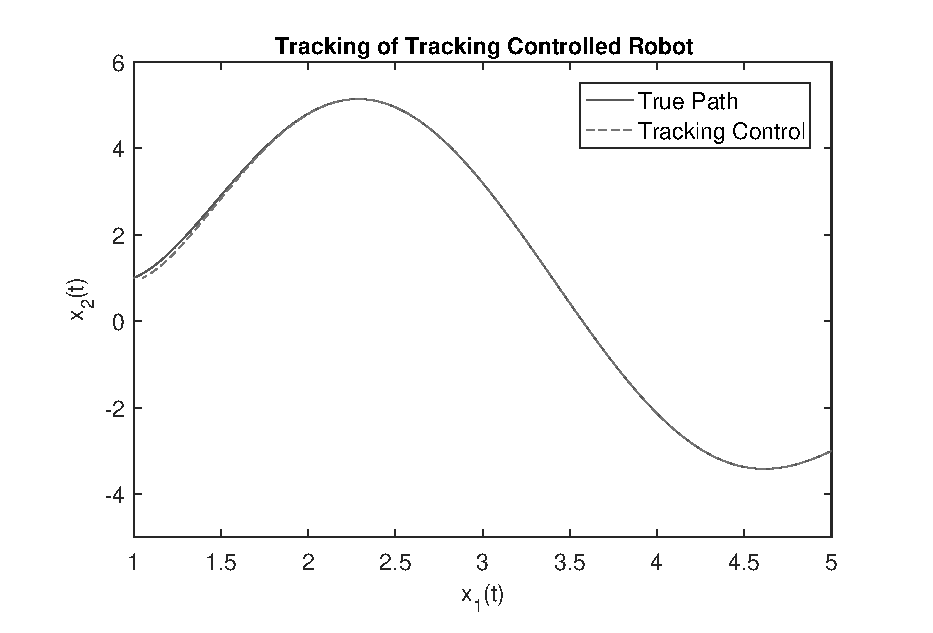
\includegraphics{images/tracking_control.eps}
    \caption{The track of the robot controlled by Tracking Control in task space. Driving towards and onto path.}
    \label{fig:track}
\end{figure}
The Serret-Frenet and Sylvester controllers should exhibit exponential convergence to the path in $\vec{\xi}$-space as the gains are chosen to satisfy the Routh-Hurwitz criterion applied to the characteristic polynomial of \eqref{eqn:tfl_control_dynamics}. Gains are specifically chosen to ensure the Serret-Frenet controller doesn't exceed an orthogonal tracking error of $0.1$, as described in Section \ref{sec:sf_stability_analysis}. The Sylvester approach uses the exact same gains to provide a fair comparison. Figure \ref{fig:tfl_compare_task} shows the resulting path of both robots in a situation where they are on the path but not facing in the right direction --- the robots start with a heading error of over 45 degrees. Notice that both methodologies converge and remain on the path no matter the behaviour of the curve.
\begin{figure}[!htbp]
    \centering
    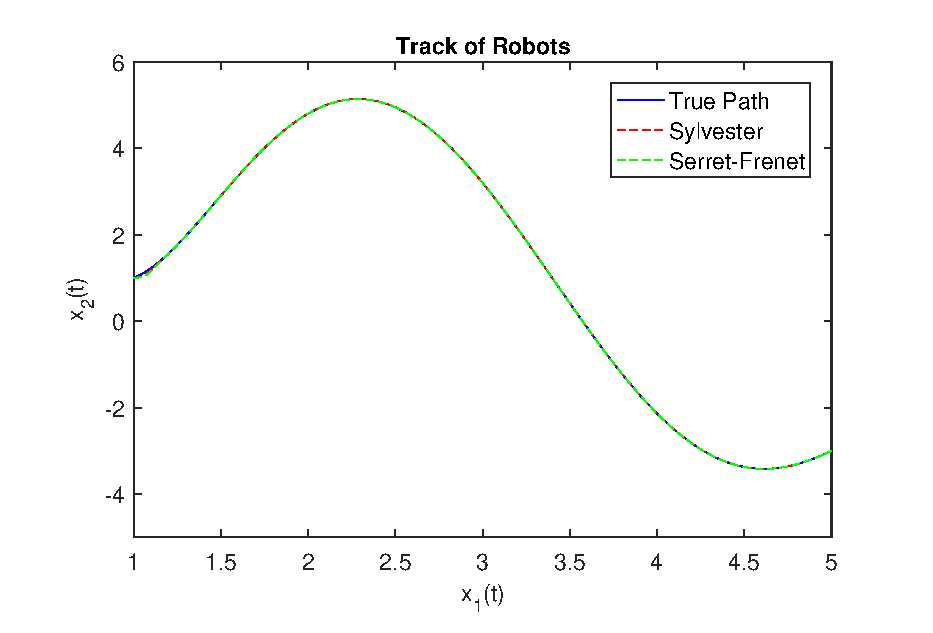
\includegraphics{images/tfl_compare_task.eps}
    \caption{The track of the robots in task space driving towards and on the path.}
    \label{fig:tfl_compare_task}
\end{figure}
Figure \ref{fig:tfl_compare_task} isn't precise enough to verify performance, so we turn to the orthogonal tracking error plot in Figure \ref{fig:tfl_compare_tracking}. It is now apparent how far away both methods go before converging to the path tangentially. Interestingly, the Sylvester controller outperforms the Serret-Frenet controller in both maximum deviation and rate of convergence. At face value, this indicates that the Sylvester controller is the one to choose.
\begin{figure}[!htbp]
    \centering
    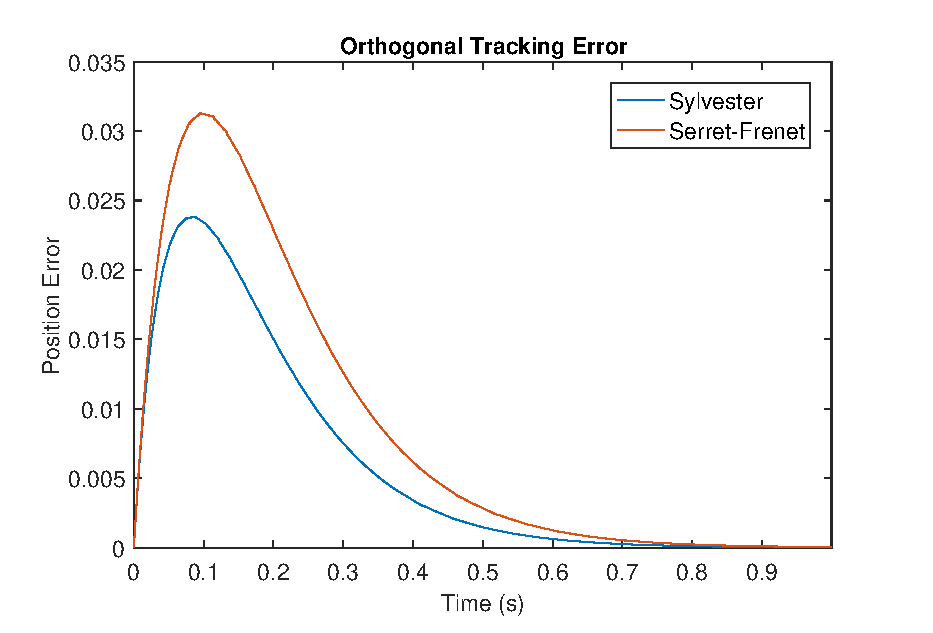
\includegraphics{images/tfl_compare_tracking.eps}
    \caption{Comparison of tracking error. Notice that both experience exponential convergence, however the Sylvester method seems to converge faster.}
    \label{fig:tfl_compare_tracking}
\end{figure}

Figure \ref{fig:tfl_compare_state} indicates a possible problem. The Sylvester controller generates states that are orders of magnitude larger than the Serret-Frenet controller, which may mean that the Sylvester controller generates large control signals. Keep in mind that the error in position was less than $10^{-1}$! However, the control signals generated are still comparable to the Serret-Frenet controller, as shown in Figure \ref{fig:control_effort}. This must mean that the Lie derivative(s) in the Sylvester method are of a similar magnitude of the state. However, there is no reason to expect this method will extend well for large polynomials over a large domain since the scaling of large magnitude states into relatively small control signals may lead to a non-negligible loss of precision. This is of serious concern for practical implementations of these controllers for high-order polynomials and/or large paths.
\begin{figure}[!htbp]
    \centering
    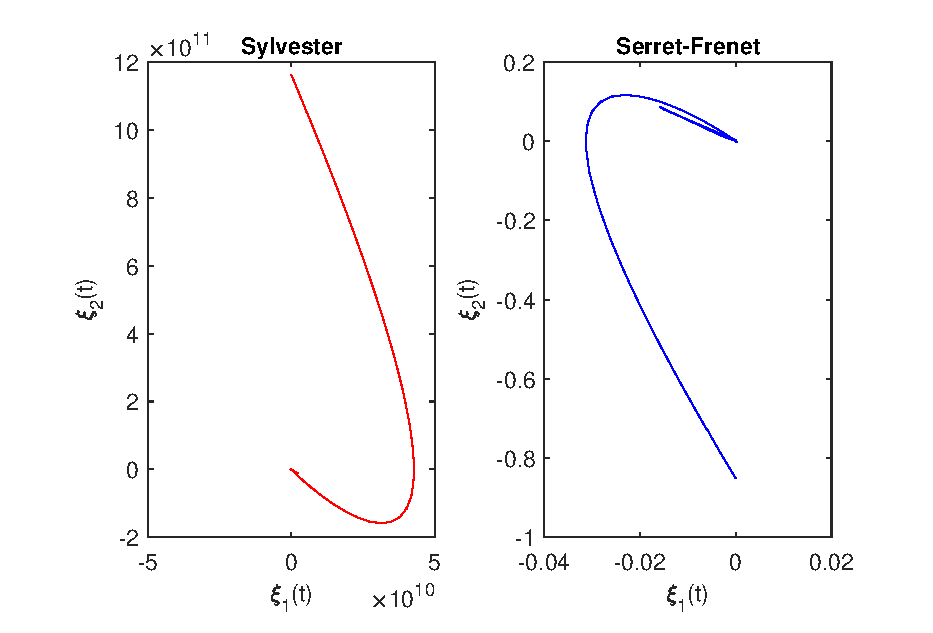
\includegraphics{images/tfl_compare_state.eps}
    \caption{The linearized state $\vec{\xi}$ for both controllers. Take careful note of the scale of the axes!}
    \label{fig:tfl_compare_state}
\end{figure}
\begin{figure}[!htbp]
    \centering
    \includegraphics{images/tfl_compare_control_signal.eps}
    \caption{Control effort of the Sylvester and Serret-Frenet controllers. They are almost indistinguishable.}
    \label{fig:control_effort}
\end{figure}

This isn't the main dimension where the Sylvester controller falls short. Table \ref{tab:perf_simple} collates the time-cost of executing the control-generation functions for both controllers, measured in MATLAB. The gradient descent algorithm is included so as to provide a useful baseline of performance. Notice that the gradient descent is the dominating cost in the Serret-Frenet controller. The Sylvester controller, on the other hand, performs poorly. In fact, data --- not shown here --- indicates that 62\% of the time is spent just calculating the $\vec{\xi}$ state vector. Any implementation of the Sylvester controller can perform, at best, around 30 steps per second. The reader would like to take note that the machine used for benchmarking uses an Intel processor running at 2.50GHz. An embedded processor is unlikely to effectively execute the Sylvester controller. Unfortunately, these are timing benchmarks and are, as a result, not easily transferable to other hardware. An analysis of floating point operations is required.
\begin{table}[!htbp]
    \centering
    \begin{tabular}{l|c|c|c}
        Function of Interest & Total Time Used (s) & Number of Calls & Estimated Cost (ms) \\ \hline
        \emph{Gradient Descent} & $11.339$ & $2017$ & $5.6217$\\ \hline
        Serret-Frenet & $12.812$ & $2017$ & $6.3520$ \\ \hline
        Sylvester & $61.338$ & $2095$ & $29.278$
    \end{tabular}
    \caption{Time cost of the control generation functions. The gradient descent algorithm cost is included in their timing results.}
    \label{tab:perf_simple}
\end{table}
Both controllers were implemented in C++ and compiled with GCC with optimization turned off in order to correctly estimate number of floating point operations. Table \ref{tab:perf_flop} lists the results. The Serret-Frenet controller is expected to be 3 orders of magnitude faster just by a rough count of floating point operations. This is a rough estimate as it doesn't account for optimization.
\begin{table}[!htbp]
    \centering
    \begin{tabular}{l|c|c}
        Function of Interest & Floating Point Operation Count & Comments\\ \hline
        Serret-Frenet & $316$ & From evaluating polynomial and its derivatives.\\  \hline
        Sylvester & $111159$ & From the level set evaluation functions.
    \end{tabular}
    \caption{Floating point operation counts. Manually counted by assembly inspection and regular expression searches, cross-verified with actual source code. Values may vary by single-digit percentiles but their order of magnitude should remain the same.}
    \label{tab:perf_flop}
\end{table}

\section{Mock World Study}
In this section, the controllers are pitted against one another in a mock real world use case. The University of Waterloo campus map was mocked, treating buildings as rectangular obstacles, as shown in Figure \ref{fig:mock_campus}. The robots begin at the bottom of campus and are told to make their way to the top of campus. An implementation of RRT is used to discover paths to the goal. The spline generated is a sequence of quintic polynomials stitched together preserving $C^2$ continuity as required. The path followed by both the Serret-Frenet controller and the Tracking controller are shown in Figures \ref{fig:mock_campus_serret_frenet} and \ref{fig:mock_campus_tracking}. The asterisks occur at points where the robot made the decision to change the path, i.e. initiate path planning.

\begin{figure}[!htbp]
    \centering
    \begin{subfigure}[t]{0.4\textwidth}
        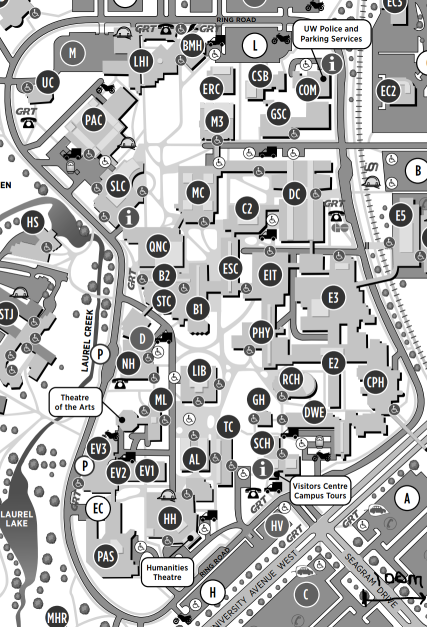
\includegraphics[width=\linewidth]{images/campus_map.PNG}
        \caption{Original campus map.}
    \end{subfigure}
    \hfill
    \begin{subfigure}[t]{0.4\textwidth}
        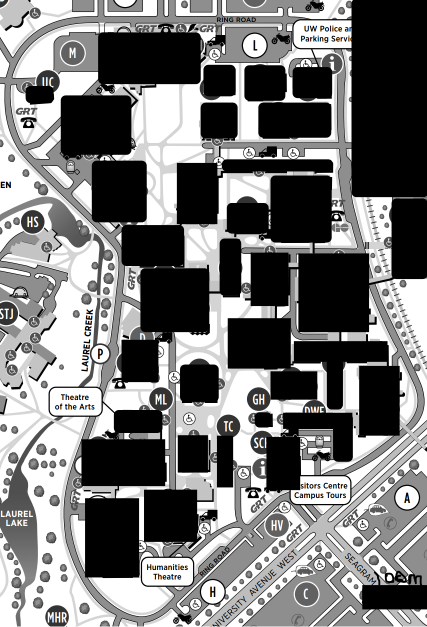
\includegraphics[width=\linewidth]{images/campus_map_block.png}
        \caption{Original campus map with rectangular obstacles.}
    \end{subfigure}
    \caption{Mock campus world model. 1 pixel equals approximately 0.64m.}
    \label{fig:mock_campus}
\end{figure}

\begin{figure}[!htbp]
    \centering
    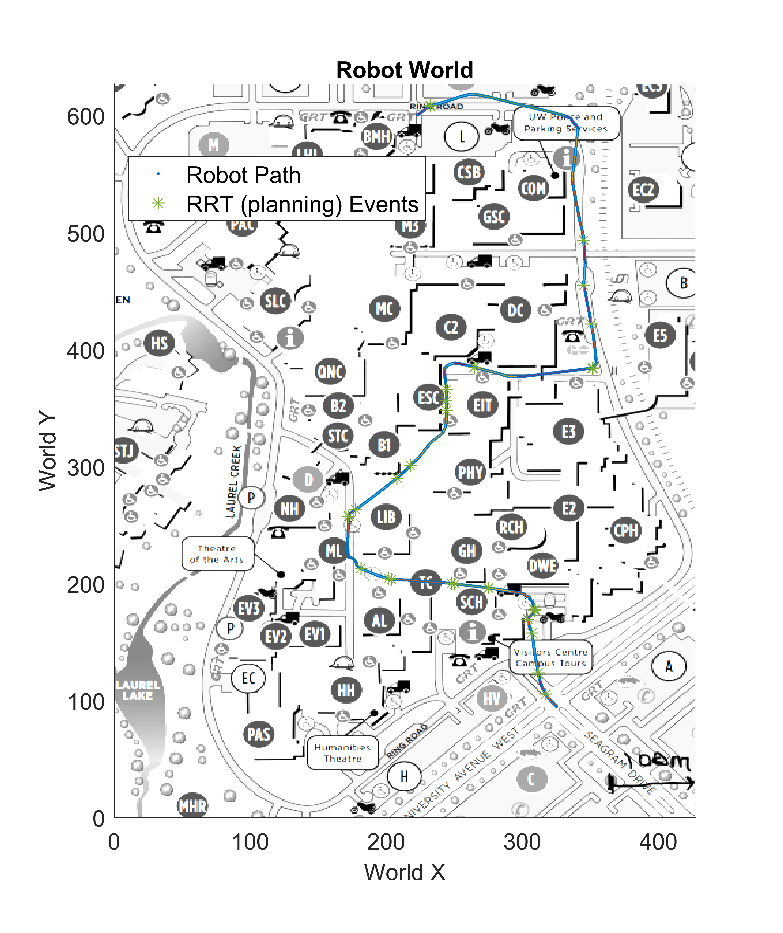
\includegraphics{images/campus_serret_frenet.eps}
    \caption{Path followed by Serret-Frenet controller.}
    \label{fig:mock_campus_serret_frenet}
\end{figure}

\begin{figure}[!htbp]
    \centering
    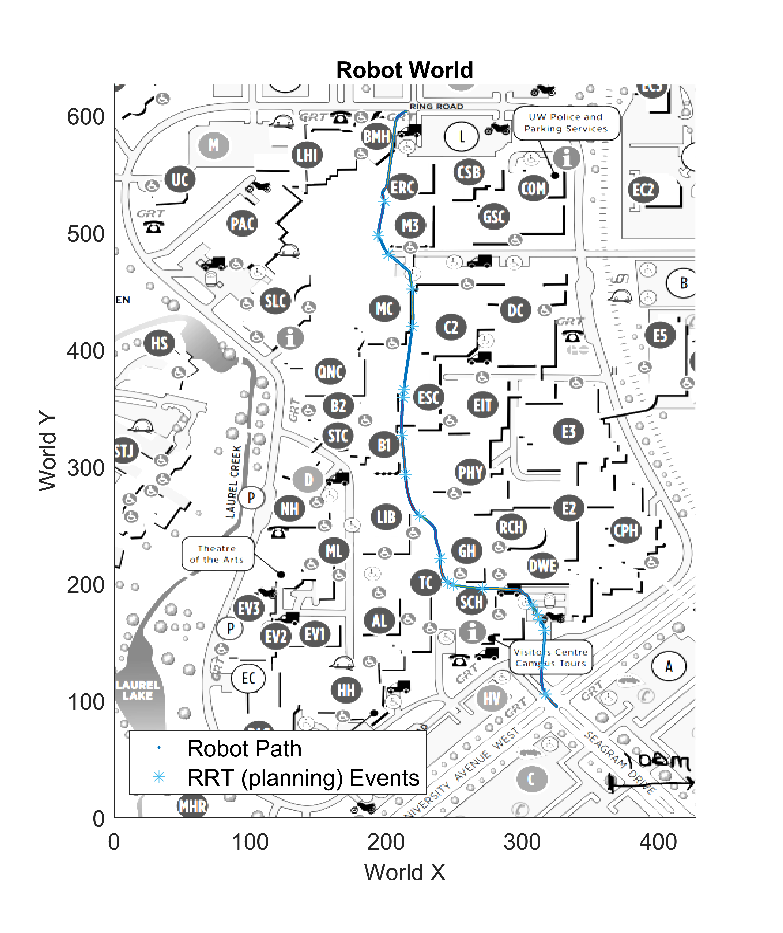
\includegraphics{images/campus_tracking.eps}
    \caption{Path followed by Tracking controller.}
    \label{fig:mock_campus_tracking}
\end{figure}
Both controllers achieve, at face value, the tracking objective. We can only know for sure by verifying the tracking error. Figures \ref{fig:mock_campus_serret_frenet_error} and \ref{fig:mock_campus_tracking_error} illustrate the tracking error. The Serret-Frenet controller maintains an almost constant error that is negligible, since the path is planned such that the robot is already correctly configured on the path. This corroborates our knowledge that the Serret-Frenet controller treats the path as invariant. The tracking controller also achieves relatively good tracking, except at the path planning event points. This may occur because the path plan begins at the robot's position, instead of the lead point. Barring this issue, the tracking controller performs well. However, notice that we can achieve just as good tracking without the velocity control introduced by the tracking controller. Moreover, the tracking controller requires a great deal of tuning.
\begin{figure}[!htbp]
    \centering
    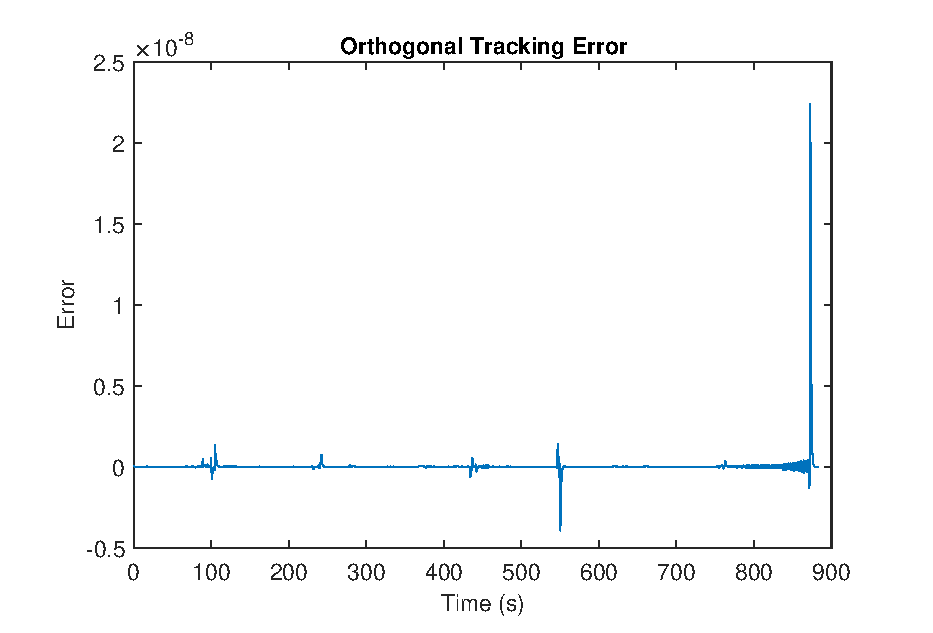
\includegraphics{images/campus_serret_frenet_error.eps}
    \caption{Error (orthogonal only) in Serret-Frenet controller.}
    \label{fig:mock_campus_serret_frenet_error}
\end{figure}
\begin{figure}[!htbp]
    \centering
    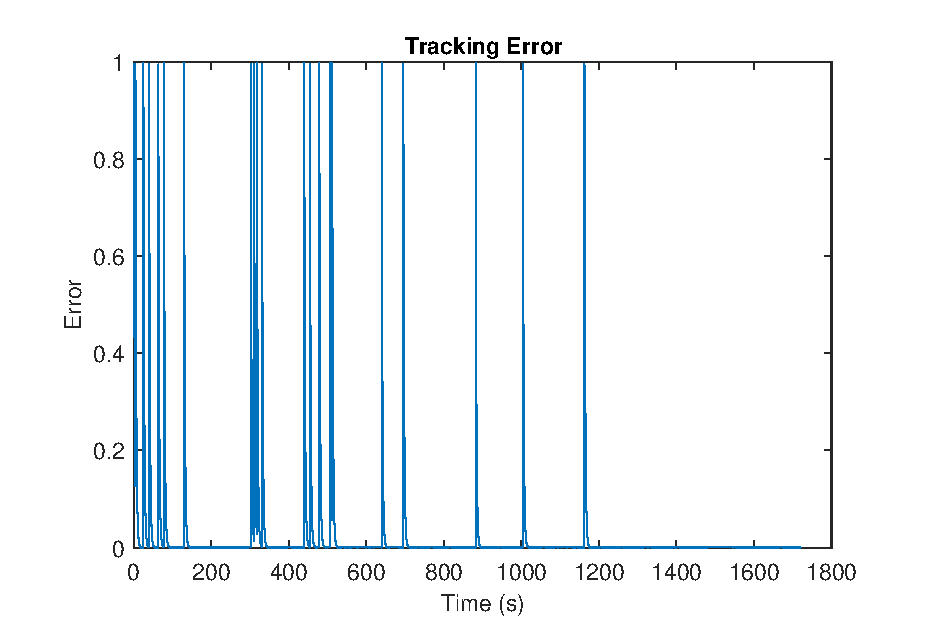
\includegraphics{images/campus_tracking_error.eps}
    \caption{Error in Tracking controller.}
    \label{fig:mock_campus_tracking_error}
\end{figure}
The reader may be wondering why the Sylvester controller was not tested in this benchmark. There are a few reasons for this:
\begin{enumerate}
    \item The control level set functions could not be optimized by the compiler (GCC).
    \item Integration tolerances could not be achieved.
\end{enumerate}
The components of $\vec{\xi}$ are at least 10 orders of magnitude larger than the Serret-Frenet controller (or, for that matter, any reasonable controller) as seen in Figure \ref{fig:tfl_compare_state}. The control signal however is still reasonable, shown in Figure \ref{fig:control_effort}, and in fact closely follows that of the Serret-Frenet controller. With that said, this controller is at risk of numerical errors due to relative magnitude of the lie derivatives/state and the resulting control signal. This may be why integration tolerances could not be achieved in the larger polynomial case.

\section{Conclusions}
A set of path following controllers were implemented in both MATLAB and C++ and verified in a relatively large scale mock example. A reformulation of the splining problem in terms of looser constraints was proposed. An analysis of the Serret-Frenet controller was performed, with the additional development a control design methodology that allows for a control engineer to design gains based on a-priori restrictions on the orthogonal tracking error.

\eqref{thm:sf_stability} does provoke a few interesting lines of research. Firstly, it motivates the use of a dynamic gain, that changes as the system evolves deeper into the invariant set. This approach may be able to speed convergence towards the path while ensuring the robot doesn't veer outside into the unknown domain. In addition to this, the Theorem seems to indicate that a design methodology may exist that incorporates conditions on $\vec{\xi}_2$ as well! Restrictions on $\vec{\xi}_2$ are effectively equivalent to preventing the robot from approaching too steeply towards the path. This may have applicability in domains where the robot cannot (and maybe even should not) make a bee-line towards the path for safety reasons. A simple example is a car which must switch from the slow lane to the fast lane on a wide highway. Even on an open road, it is safer for both passengers and other drivers to approach in a manner that reduces the turn rate.

The Sylvester controller, though mathematically elegant, doesn't seem to be well suited for practical implementation. In fact, my compiler couldn't optimize any of the Lie derivative and Level set functions for the Sylvester controller. Instead, the compiler hung. This and the fact that the Sylvester controller is expensive in terms of floating point operations, indicates a lack of practicality. Even in simulation, the Sylvester controller generated unreasonably large linearized states that were then scaled down with possible loss of precision. It is apparent that the Serret-Frenet controller is superior.

\backmatter
\cleardoublepage
\phantomsection
\addcontentsline{toc}{chapter}{References}
\markright{\textsc{References}}
\printbibliography[title=References]

\cleardoublepage
\phantomsection
\addcontentsline{toc}{chapter}{Index}
\markright{\textsc{Index}}
\printindex

\end{document}
